\documentclass[paper=a4, fontsize=11pt]{scrartcl} % A4 paper and 11pt font size

\newcommand{\assignment}{4}
\newcommand{\duedate}{March 1, 2023}
\usepackage[top=1in, bottom=1.5in, left=1in, right=1in]{geometry}
\usepackage{fancyhdr} % Required for custom headers
\usepackage{lastpage} % Required to determine the last page for the footer
\usepackage{extramarks} % Required for headers and footers
\usepackage[usenames,dvipsnames]{color} % Required for custom colors
\usepackage{graphicx} % Required to insert images
\usepackage{listings} % Required for insertion of code
\usepackage{courier} % Required for the courier font
\usepackage{amsmath}
\usepackage[super]{nth}
\usepackage{booktabs}
\usepackage[usenames,dvipsnames]{xcolor}
\usepackage{tcolorbox}
\usepackage{tabularx}
\usepackage{array}
\usepackage{colortbl}

%\usepackage[T1]{fontenc} % Use 8-bit encoding that has 256 glyphs
%\usepackage{fourier} % Use the Adobe Utopia font for the document - comment this line to return to the LaTeX default
\usepackage[english]{babel} % English language/hyphenation
\usepackage{amsmath,amsfonts,amsthm} % Math packages
\usepackage{graphicx}

\usepackage{hyperref}
\hypersetup{
  colorlinks   = true, %Colours links instead of ugly boxes
  urlcolor     = blue, %Colour for external hyperlinks
  linkcolor    = blue, %Colour of internal links
  citecolor   = red %Colour of citations
}

\usepackage{fancyhdr} % Custom headers and footers
\pagestyle{fancyplain} % Makes all pages in the document conform to the custom headers and footers
\fancyhead{} % No page header - if you want one, create it in the same way as the footers below
\fancyfoot[L]{} % Empty left footer
\fancyfoot[C]{} % Empty center footer
\fancyfoot[R]{\thepage} % Page numbering for right footer
\renewcommand{\headrulewidth}{0pt} % Remove header underlines
\renewcommand{\footrulewidth}{0pt} % Remove footer underlines
\setlength{\headheight}{13.6pt} % Customize the height of the header
\newcommand{\ts}{\textsuperscript}

\numberwithin{equation}{section} % Number equations within sections (i.e. 1.1, 1.2, 2.1, 2.2 instead of 1, 2, 3, 4)
\numberwithin{figure}{section} % Number figures within sections (i.e. 1.1, 1.2, 2.1, 2.2 instead of 1, 2, 3, 4)
\numberwithin{table}{section} % Number tables within sections (i.e. 1.1, 1.2, 2.1, 2.2 instead of 1, 2, 3, 4)

\setlength\parindent{0pt} % Removes all indentation from paragraphs - comment this line for an assignment with lots of text

% Default fixed font does not support bold face
\DeclareFixedFont{\ttb}{T1}{txtt}{bx}{n}{8} % for bold
\DeclareFixedFont{\ttm}{T1}{txtt}{m}{n}{8}  % for normal

%----------------------------------------------------------------------------------------
%	CODE BLOCKS
%----------------------------------------------------------------------------------------

\usepackage{adjustbox}
\usepackage{listings}
\usepackage{color}

\definecolor{dkgreen}{rgb}{0,0.6,0}
\definecolor{gray}{rgb}{0.5,0.5,0.5}
\definecolor{mauve}{rgb}{0.58,0,0.82}

\lstdefinelanguage{Dockerfile}
{
  morekeywords={FROM, RUN, CMD, LABEL, MAINTAINER, EXPOSE, ENV, ADD, COPY,
    ENTRYPOINT, VOLUME, USER, WORKDIR, ARG, ONBUILD, STOPSIGNAL, HEALTHCHECK,
    SHELL},
  morecomment=[l]{\#},
  morestring=[b]"
}

\lstset{
    columns=flexible,
    aboveskip=5mm,
    belowskip=5mm,
    keepspaces=true,
    showstringspaces=false,
    basicstyle=\ttfamily,
    commentstyle=\color{gray},
    keywordstyle=\color{purple},
    stringstyle=\color{green}
}



%----------------------------------------------------------------------------------------
%	TITLE SECTION
%----------------------------------------------------------------------------------------

\usepackage{eso-pic}
% \usepackage[demo]{graphicx}
\newcommand\AtPageUpperRight[1]{\AtPageUpperLeft{%
   \makebox[\paperwidth][r]{#1}}}

\newcommand{\horrule}[1]{\rule{\linewidth}{#1}} % Create horizontal rule command with 1 argument of height

\title{	
\normalfont \normalsize
\textsc{Northeastern University,  Khoury College of Computer Science} \\ [25pt] % Your university, school and/or department name(s)
\horrule{0.5pt} \\[0.4cm] % Thin top horizontal rule
\huge CS 6220  Data Mining \textemdash~Assignment \assignment \\ % The assignment title
\Large \textbf{Due: \duedate (100 points)} % The assignment title
\horrule{2pt} \\[0.5cm] % Thick bottom horizontal rule
}

% Original in the document
\AddToShipoutPictureBG*{%
  \AtPageUpperRight{\raisebox{-\height}{
\includegraphics[width=3cm]{include/logo}}}}

\author{
    \textbf{YOUR NAME} \\ 
    \textbf{YOUR GIT USERNAME} \\ 
    \textbf{YOUR E-MAIL}
}% INFORMATION

\date{} % Today's date or a custom date

\author{
    \textbf{YOUR NAME} \\ 
    \textbf{YOUR GIT USERNAME} \\ 
    \textbf{YOUR E-MAIL}
}% INFORMATION

\begin{document}

\maketitle % Print the title

{\huge \textbf{K-Means}} \\

The~\href{https://course.ccs.neu.edu/cs6220/homework-4/data/}{normalized automobile distributor timing speed and ignition coil gaps} for production F-150 trucks over the years of 1996, 1999, 2006, 2015, and 2022. We have stripped out the labels for the five years of data.\\
\\
Each sample in the dataset is two-dimensional, i.e. $\textbf{x}_i \in \mathbb{R}^2$ (one dimension for timing speed and the other for coil gaps), and there are $N=5000$ instances in the data.
\\

{\Large \textbf{Question 1} [20 pts total]} \\

\textbf{[10 pts] Question 1a.)} Implement a simple $k$-means algorithm in Python on Colab with the following initialization:

\begin{equation}
\textbf{x}_1 = \left( \begin{matrix} 10 \\ 10 \end{matrix} \right), \textbf{x}_2 = \left( \begin{matrix} -10 \\ -10 \end{matrix} \right),
\textbf{x}_3 = \left( \begin{matrix} 2 \\ 2 \end{matrix} \right),
\textbf{x}_4 = \left( \begin{matrix} 3 \\ 3 \end{matrix} \right),
\textbf{x}_5 = \left( \begin{matrix} -3 \\ -3 \end{matrix} \right),
\nonumber
\end{equation} \\

You need only 100 iterations, maximum, and your algorithm should run very quickly to get the results. \\
\begin{verbatim}
def my_kmeans(xs: np.ndarray, init_centers: np.ndarray, n_iter=100):
    N,D = xs.shape
    K = init_centers.shape[0]
    final_centers = init_centers
    for it in range(n_iter):
        dist = cdist(xs,final_centers)
        cluster_id = np.argmin(dist,axis=1)
        for i in range(K):
            final_centers[i,:] = np.mean(xs[cluster_id==i],axis=0)    
            
    dist = cdist(xs,final_centers)
    cluster_id = np.argmin(dist,axis=1)
    return final_centers,cluster_id
\end{verbatim}

\textbf{[5 pts] Question 1b.)} Scatter the results in two dimensions with different clusters as different colors. You can use \textbf{matplotlib}'s \textbf{pyplot} functionality:

\begin{verbatim}
import matplotlib.pyplot as plt
data = np.array([[10,10],[-10,-10],[2,2],[3,3],[-3,-3]])
centroids,cluster_id = my_kmeans(x,data)
plt.scatter(x[:,0],x[:,1],c=cluster_id)
plt.scatter(centroids[:,0],centroids[:,1],c='r')
plt.show()
\end{verbatim}

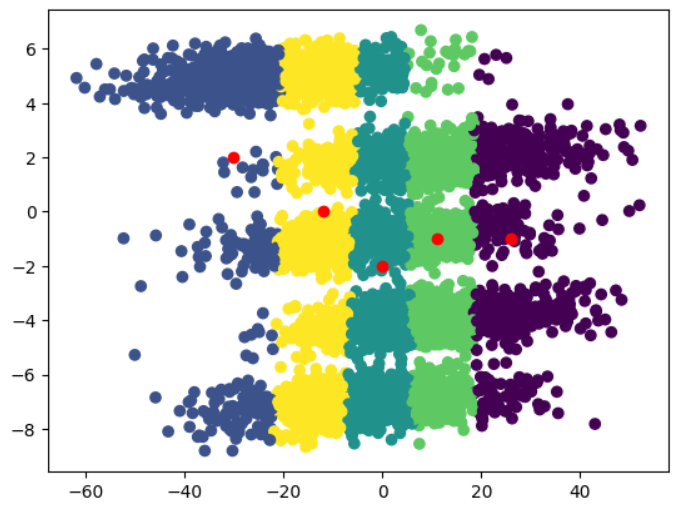
\includegraphics{include/k-means_cluster.png}

\textbf{[5 pts] Question 1c.)} You will notice that in the above, there are only five initialization clusters. Why is $k=5$ a logical choice for this dataset? After plotting your resulting clusters, what do you notice? Did it cluster very well? Is there an initialization that would make it cluster well?\\
\\
From the data scatter plot, we can see that the data's distribution are five short strips and each strip is a cluster. Therefore, we choose k=5 as the clustering number. 


When we draw the resulting clusters, we can see that the result breaks the original distribution of data and it cuts each strip into five parts. Therefore, it doesn't cluster well.


There doesn't exist an initialization that would make it cluster well. Kmeans can't do well in such shape of data. \\
\\
{\Large \textbf{Question 2)}[30 pts total]} \\

In the data from Question 1, let \textbf{x} and \textbf{y} be two instances, i.e., they are each truck with separate measurements.  A common distance metric is the \emph{Mahalanobis Distance} with a specialized matrix $P \in \mathbb{R}^{2 \times 2}$ that is written as follows: 

\begin{equation}
d(\textbf{x}, \textbf{y}) = ( \textbf{x} - \textbf{y} )^T P^{-1} ( \textbf{x} - \textbf{y} )
\nonumber
\end{equation} \\

In scalar format (non-matrix format), the Mahalanobis Distance can be expressed as:

\begin{equation}
    d(\textbf{x}, \textbf{y}) = \sum_{i=1}^2 \sum_{j=1}^2 (x_i - y_i) \cdot P^{-1}_{i,j} \cdot (x_j - y_j)
    \nonumber
\end{equation}

where \textbf{x} and \textbf{y} are two instances of dimensionality 2, and $d(\textbf{x}, \textbf{y})$ is the distance between them. In the case of the F150 engine components, $P$ is a known relationship through Ford's quality control analysis each year, where it is numerically shown as below: \\

\begin{equation}
 P = \left(
\begin{matrix}
10 & 0.5 \\
-10 & 0.25
\end{matrix}
\right) \nonumber
\end{equation}
\\

\textbf{[15 pts] Question 2a.)} Using the same data as \textbf{Question 1} and the same initialization instances $\{\textbf{x}_1, \textbf{x}_2, \textbf{x}_3, \textbf{x}_4, \textbf{x}_5 \}$ implement a specialized $k$-means with the above Mahalanobis Distance. Scatter the results with the different clusters as different colors. \\

What do you notice? You may want to pre-compute $P^{-1}$ so that you aren't calculating an inverse every single loop of the the $k$-Means algorithm. 
\begin{verbatim}
def new_kmeans(xs, init_centers, VI, n_iter=100):
    N,D = xs.shape
    K = init_centers.shape[0]
    final_centers = init_centers
    
    for it in range(n_iter):
        dist = cdist(xs,final_centers,metric='mahalanobis', VI=VI)
        cluster_id = np.argmin(dist,axis=1)
            
        for i in range(K):
            final_centers[i,:] = np.mean(xs[cluster_id==i],axis=0)    
            
    dist = cdist(xs,final_centers,metric='mahalanobis', VI=VI)
    cluster_id = np.argmin(dist,axis=1)
    return final_centers,cluster_id
p = np.array([[10,0.5],[-10,0.25]])
inv_p = np.linalg.inv(p)
data = np.array([[10,10],[-10,-10],[2,2],[3,3],[-3,-3]])
new_centroids,new_cluster_id = new_kmeans(x,data,VI=inv_p)
\end{verbatim}
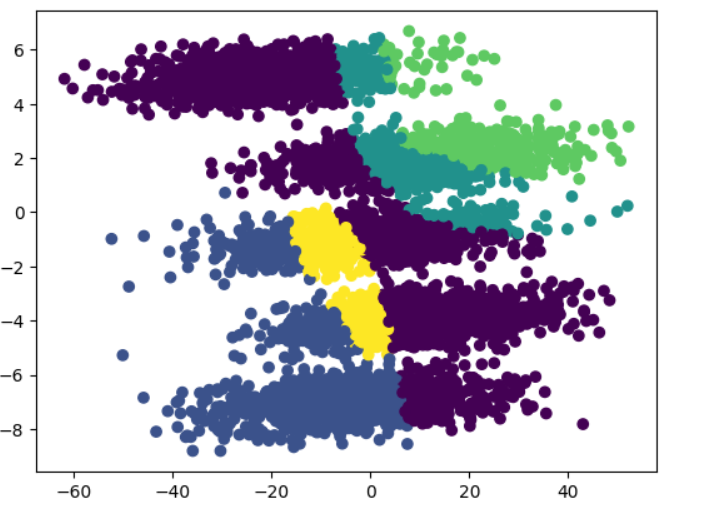
\includegraphics{include/new_kmeans_cluster.png}

\textbf{[5 pts] Question 2b.)}
Calculate and print out the principle components of the aggregate data. \\

1st pc is [-0.99838317,  0.05684225], \\
2nd pc is [-0.05684225, -0.99838317]
\\ \\
\textbf{[5 pts] Question 2c.)}
Calculate and print out the principle components of \emph{each cluster}. Are they the same as the aggregate data? Are they the same as each other?\\

For cluster 0,the compenents are:[[-0.98439765,  0.17595815]
 [-0.17595815, -0.98439765]]  \\
For cluster 1,the compenents are:[[-0.9966809,   0.08140747]
 [ 0.08140747,  0.9966809 ]]   \\
For cluster 2,the compenents are:[[ 0.99089241, -0.13465595]
 [ 0.13465595,  0.99089241]]   \\
For cluster 3,the compenents are:[[ 0.99902772, -0.04408651]
 [ 0.04408651,  0.99902772]]   \\
For cluster 4,the compenents are:[[-0.97099153,  0.23911388]
 [ 0.23911388,  0.97099153]]   \\

 They are not same as the aggregate data. And they are also different from each other.\\

 
\textbf{[5 pts] Question 2d.)}
Take the eigenvector / eigenvalue decomposition of $P^T$ and subsequently, take their product. That is to say, 

\begin{equation}
    \{\Lambda, \Phi\} = \verb"eig"\left( P^T \right)
    \nonumber
\end{equation}

where $\Lambda = \left( \begin{matrix} \lambda_1 & 0 \\ 0 & \lambda_2 \end{matrix} \right)$ and $\Phi$ is a $2 \times 2$ matrix with $\phi_i \in \mathbb{R}^2$, a column in $\Phi$. Calculate a new $P'$ such that

\begin{equation}
    P' = \Lambda \Phi \nonumber
\end{equation}
\\
What is the relationship between $P'$ and the data? 
\\
Throug coding, we obtain $\Lambda = \left( \begin{matrix} 9.45693086 & 0 \\ 0 & 0.79306914 \end{matrix} \right)$. The new $P'=\left(\begin{matrix}
    9.44301625 & 6.95724558\\
    0.04300577 & 0.53717161 \\
\end{matrix}  \right)$


\vspace{10mm}

{\huge \textbf{Market Basket Analysis and Algorithms}} \\

Consider $F_3$ as the following set of frequent 3-itemsets:

\begin{verbatim}
{1, 2, 3}, {1, 2, 4}, {1, 2, 5}, {1, 3, 4}, 
{2, 3, 4}, {2, 3, 5}, {3, 4, 5}.
\end{verbatim} \\

Assume that there are only five items in the data set. \\

{\Large \textbf{Question 3} [25 pts total]} \\
\\
\textbf{[10 pts] Question 3a.)} List all candidate 4-itemsets obtained by a candidate generation procedure using the $F_{k - 1} \times F_1$ merging strategy. 
\begin{verbatim}
{1,2,3,4}, 
{1,2,3,5},
{1,2,4,5},
{1,3,4,5},
{2,3,4,5}
\end{verbatim} 
\\

\textbf{[10 pts] Question 3b.)} List all candidate 4-itemsets obtained by the candidate generation procedure in A Priori, using $F_{k-1} \times F_{k-1}$. 
\begin{verbatim}
{1,2,3,4},
{1,2,3,5},
{1,2,4,5},
{2,3,4,5}
\end{verbatim} 
\\

\textbf{[5 pts] Question 3c.)} List all candidate 4-itemsets that survive the candidate pruning step of
the Apriori algorithm. \\
\\
\{1,2,3,5\}'s subset \{1,3,5\} is not in $F_3$, therefore, it will be pruned.\\
\{1,2,4,5\}'s subset \{1,4,5\},\{2,4,5\} are not in $F_3$, therefore, it will be pruned. \\
\{2,3,4,5\}'s subset \{2,4,5\} is not in $F_3$, therefore, it will be pruned.

Therefore, the survived candidate is \{1,2,3,4\}.


\vspace{10mm}

{\Large \textbf{Question 4} [25 pts total]} \\
 
Consider the following table for questions 4a) to 4c):\\
\begin{center}
\begin{tabular}{ll}
Transaction ID & Items \\
\rowcolor[HTML]{DEEBF6} 
\textbf{1}     & \textbf{\{Beer, Diapers\}} \\
\rowcolor[HTML]{DEEBF6} 
\textbf{2}     & \textbf{\{Milk, Diapers, Bread, Butter\}} \\
\rowcolor[HTML]{DEEBF6} 
\textbf{3}     & \textbf{\{Milk, Diapers, Cookies\}} \\
\rowcolor[HTML]{DEEBF6} 
\textbf{4}     & \textbf{\{Bread, Butter, Cookies\}} \\
\rowcolor[HTML]{DEEBF6} 
\textbf{5}     & \textbf{\{Milk, Beer, Diapers, Eggs\}} \\
\rowcolor[HTML]{DEEBF6} 
\textbf{6}     & \textbf{\{Beer, Cookies, Diapers\}} \\
\rowcolor[HTML]{DEEBF6} 
\textbf{7}     & \textbf{\{Milk, Diapers, Bread, Butter\}} \\
\rowcolor[HTML]{DEEBF6} 
\textbf{8}     & \textbf{\{Bread, Butter, Diapers\}} \\
\rowcolor[HTML]{DEEBF6} 
\textbf{9}     & \textbf{\{Bread, Butter, Milk\}} \\
\rowcolor[HTML]{DEEBF6} 
\textbf{10}    & \textbf{\{Beer, Butter, Cookies\}}    
\end{tabular}
\end{center}

\vspace{8mm}

\textbf{[3 pts] Question 4a.)} What is the maximum number of association rules that can be extracted from this data (including rules that have zero support)? \\
There are 7 unique items. Therefore, the maximum number of association rules is $3^7 - 2^8 +1=1932$\\

\textbf{[3 pts] Question 4b.)} What is the confidence of the rule $\{ \text{Milk, Diapers} \} \Rightarrow \{ \text{Butter} \}$? \\
$$
confidence=\frac{\sigma(\{Milk,Diaper,Butter\})}{\sigma(\{Milk,Diaper\})}\\
=\frac{2}{4}=0.5
$$


\textbf{[3 pts] Question 4c.)} What is the support for the rule $\{ \text{Milk, Diapers} \} \Rightarrow \{ \text{Butter} \}$? \\

$$
support = \frac{\sigma(\{Milk,Diapers,Butter\})}{|T|} \\
=\frac{2}{10} = 0.5\\
$$

\textbf{[3 pts] Question 4d.)} \verb"True" or \verb"False" with an explanation: Given that \{a,b,c,d\} is a frequent itemset, \{a,b\} is always a frequent itemset. \\
True. \\
$\{a,b\}\in \{a,b,c,d\}$, that means $support(\{a,b\})\geq support(\{a,b,c,d\})$. Therefore, when $\{a,b,c,d\}$ is a frequent itemset, $\{a,b\}$ is also a frequent itemset.\\



\textbf{[3 pts] Question 4e.)} \verb"True" or \verb"False" with an explanation: Given that \{a,b\}, \{b,c\} and \{a,c\} are frequent itemsets, \{a,b,c\} is always frequent. \\
False.\\
For example, when  \{a,b\}, \{b,c\} and \{a,c\} are frequent itemsets, the itemsets \{a,b,c\} may not occur in the transactions. At this time, its support is 0. Certainly, it's not a frequent itemset. \\ 


\textbf{[3 pts] Question 4f.)} \verb"True" or \verb"False" with an explanation: Given that the support of \{a,b\} is 20 and the support of \{b,c\} is 30, the support of \{b\} is larger than 20 but smaller than 30. \\
False.      \\
The support of \{b\} is at least larger than $20+30=50$. \\


\textbf{[3 pts] Question 4g.)} \verb"True" or \verb"False" with an explanation: In a dataset that has 5 items, the maximum number of size-2 frequent itemsets that can be extracted (assuming minsup $> 0$) is 20. \\
False. \\
The maximum number is $\binom{5}{2}=10$ \\

\textbf{[4 pts] Question 4h.)} Draw the itemset lattice for the set of unique items $\mathcal{I} = \{ a, b, c \}$. \\

\begin{center}
    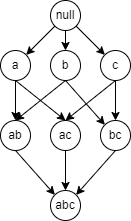
\includegraphics[width=75mm]{include/itemset lattice.png}
\end{center}

\end{document}
